% ---------------------------------------------------------------------
% EG author guidelines plus sample file for EG publication using LaTeX2e input
% D.Fellner, v1.17, Sep 23, 2010


\title{Minimal Energy Based Hybrid Model For Multi-Agent Simulations}

% for anonymous conference submission please enter your SUBMISSION ID
% instead of the author's name (and leave the affiliation blank) !!
\author{Haiying Liu\thanks{e-mail:lhysunshine@gmail.com}\\Beijing Institute of Technology}


\begin{document}

% \teaser{
%  
\includegraphics[width=\linewidth]{eg_new}
%  \centering
%   \caption{New EG Logo}
% \label{fig:teaser}
% }

\maketitle

\begin{abstract}
   The behavior of large human crowd is very complicated and subtle due to complex local collision strategies for dynamic crowd density distribution in the scene. We present a hybrid approach to simulate complex crowd behavior by combining continuous crowd algorithm and agent-based algorithm. For dense groups, we introduce a minimal-energy method to minimize conflict between dense groups and constrain the maximum density of each grid; For sparse groups, we adapt RVO algorithm to simulate agent-agent and agent-group interactions.

\begin{classification} % according to http://www.acm.org/class/1998/
\CCScat{Computer Graphics}{I.3.7}{Three-Dimensional Graphics and Realism}{Animation}
\end{classification}

\end{abstract}





%-------------------------------------------------------------------------
\section{Introduction}

Please follow the steps outlined in this document very carefully when
submitting your manuscript to Eurographics.

You may as well use the \LaTeX\ source as a template to typeset your own
paper. In this case we encourage you to also read the \LaTeX\ comments
embedded in the document.

%-------------------------------------------------------------------------
\section{Related Work}

\section{Dense Crowd Flow Energy Minimization}

In this section, we introduce our approach of minimizing collision energy of dense crowds. In the observation of dense crowds behavior, groups of agents have inter-group collision, merging and negotiation while the freedom of movement of individual agents are reduced\cite{Treuille:2006,Narain:2009,Golas:2013}. Based on the observation, we define two types of collision energy, inter-group and inter-agent collision energy. We use the continuous dense crowd model from \cite{Narain:2009} to represent and minimize inter-agent collision behavior(\S\ref{section:3.1}). We develop our inter-group energy model and employ Graph Cut to minimize inter-group collision energy(\S\ref{section:3.2}). Besides, we introduce a series of constraints to limit maximum density of each group(\S\ref{section:3.3}). 

\subsection{Dense Crowd Representation}
\label{section:3.1}
Like \cite{Narain:2009}, we first use Navigation Mesh as global planning algorithm for each agent(see for details). Then, the information of discrete agents is transfered to grids by the particle-in-cell method of fluid simulation \cite{Narain:2009}. The density $\rho$ and velocity $\bar{\textbf{v}}$ can be computed as,
\begin{equation}
\label{eq:1}
 \rho(\textbf{x}) = \sum_{i} \omega_\textbf{x}(\textbf{x}_i)m_i
\end{equation}
\begin{equation}
\label{eq:2}
 \bar{\textbf{v}}(\textbf{x}) = \frac{\sum_{i} \omega_\textbf{x}(\textbf{x}_i)\tilde{\textbf{v}}_i}{\sum_{i} \omega_\textbf{x}(\textbf{x}_i)}
\end{equation} 
where $\textbf{x}_i$ is the position of the agent, $\tilde{\textbf{v}}_i$ is the prefered velocity of the agent, $m_i$ is the mass of each agent which are unity. $\omega_\textbf{x}(\textbf{x}_i)$ is the bilinear interpolation weight associated with the agent position.

After the crowd is converted to continuous representation, we can refine the crowd information by minimizing the inter-group collision energy descripted in (\S\ref{section:3.2} and \S\ref{section:3.3}).

Then, the density $\rho(\textbf{x}_i)$ and velocity $\textbf{v}(\textbf{x}_i)$ at agent position can be interpolated from grid density and grid velocity with the same method mentioned in \cite{Treuille:2006}. We can get the final velocity of each agent by interpolation between the continuum velocity $\textbf{v}(\textbf{x}_i)$ and the agent's prefered velocity $\tilde{\textbf{v}}_i$, depending on the crowd density $\rho(\textbf{x}_i)$ at its location:
\begin{equation}
\label{eq:3}
\textbf{v}_i = \tilde{\textbf{v}}_i + \frac{\rho(\textbf{x}_i)}{\rho_{max}}(\textbf{v}(\textbf{x}_i) - \tilde{\textbf{v}}_i)
\end{equation}

\subsection{Energy Minimization Model}
\label{section:3.2}
According to our observation of dense crowd behavior, collisions, merging and negotiations happen between agent groups in dense crowds. However, not like local collision avoidance strategies for agents which can be considered as rigid-body, groups are highly influenced by neighbor groups and have the trend of sharing the same movement. Inspired by the observation, we develop a minimal energy model to describe and solve inter-group collision problem.

\begin{figure}
\centering
  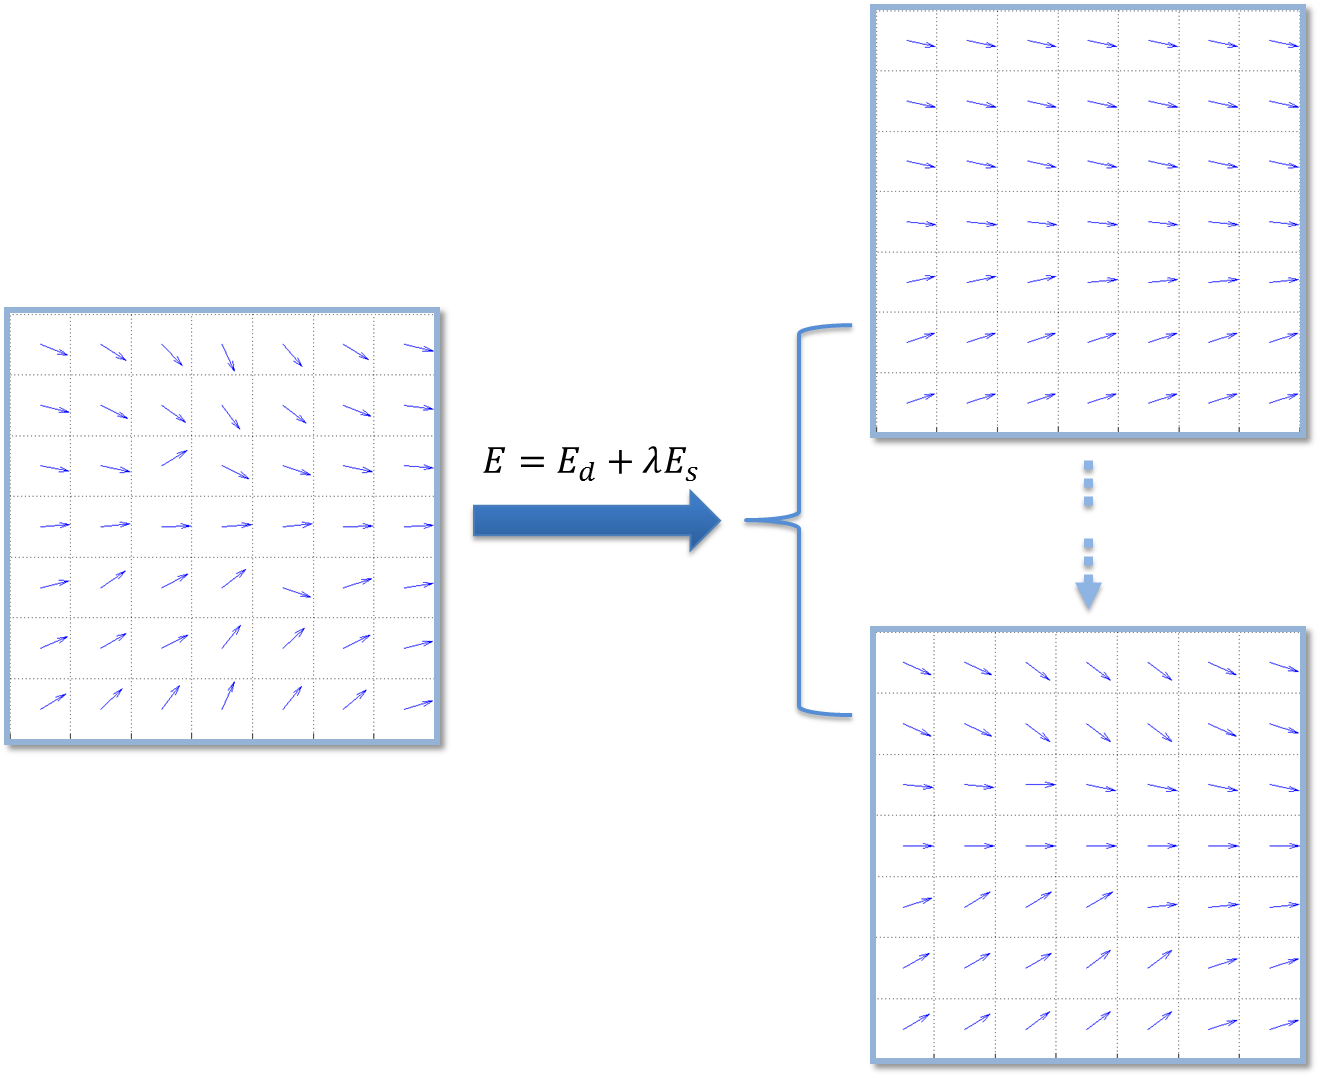
\includegraphics[width=3in]{images/energy}
  \caption{Minimal-Engergy Process Illustration. The left image is group of dense grids with grid velocities. Images on the right side are grids with refined velocities. From right-top to right-bottom, the $\lambda$ of smooth term decreased which means each grid is less influenced by neighbor grids.}
\end{figure}
We define the inter-group collision problem as a labelling problem by assigning to each grid $i$ a label $l_i$. Each grid maps to a group of agent and the number of grids are $n$. By dividing space into $m$ pieces, we can have $m$ labels, each of them represent a range of angle in the space. The energy function $E$, composed of a data energy $E_d$ and a smoothness energy $E_s$, is defined as:
\begin{equation}
\label{eq:4}
E = E_d + \lambda E_s
\end{equation}

The data energy $E_d$ is the sum of data cost of each grid with a label $d_i(l_i)$. In our energy model, the data cost $d_i(l_i)$ is defined as the angular distance from the average grid velocity $\bar{\textbf{v}}(\textbf{x})$ to the velocity of selected label $\hat{\textbf{v}}(l_i)$, which means the effort of the group to change it's velocity to negotiate with neighbor groups. We first normalize the two velocities and use the dot value of them in our implementation instead of computing angular difference as equation \ref{eq:6}.
\begin{equation}
\label{eq:5}
E_d = \sum_{i}d_i(l_i)
\end{equation}

\begin{equation}
\label{eq:6}
d_i(l_i) = 1 - \bar{\textbf{v}}(\textbf{x}) \cdot \hat{\textbf{v}}(l_i)
\end{equation}

The smoothness energy $E_s$ represent the velocity difference between neighbor grids. We use standard 4 neighbor system for dense grids, so that the smoothness energy is the sum of spacially varying horizontal and vertical neighbor smoothness costs $V_{ij}(l_i,l_j)$, where if $i=(p,q)$ and $j=(s,t)$ then $\left|p-s\right| + \left|q-t\right| = 1$. Let $\mathcal{N}$ denotes the set of all such neighboring grid pairs, the smoothness energy is
\begin{equation}
\label{eq:7}
E_s = \sum\limits_{\left\{ {i,j} \right\} \in \mathcal{N}} \omega_{ij} \cdot V(\left|l_i,l_j\right|)
\end{equation}

In equation \ref{eq:7}, $V(\left|l_i,l_j\right|)$, also can be written as $V(\Delta l)$, is a non-decreasing fundtion of the label difference, and can be directly computed as absolute differenct between two labels. $\omega_{ij}$ is a per-pair weight for $i$th and $j$th grid, which is normalized by the minimum density of a dense grid $\rho_{min}$ and the maximum density $\rho_{max}$ (see equation \ref{eq:8}). In our model, $V(\left|l_i,l_j\right|)$ is adapted to restrict the maximum density of each group(\S\ref{section:3.3}).
\begin{equation}
\label{eq:8}
\omega_{ij} = \frac{(\rho_i - \rho_{min})(\rho_j - \rho_{min})}{(\rho_{max} - \rho_{min})^2}
\end{equation}

With the definition of energy function $E$, we can use Graph Cut or Belief Propagation algorithms to compute labels for each grid to achieve the minimal energy cost. In our implementation, we use the Graph Cut implementation from \cite{Boykov:2001,Boykov:2004,Kolmogorov:2004}.

\subsection{Constraints}
\label{section:3.3}
While trying to reach the minimal energy cost of inter-group collision, we should also keep the density of each group below the maximum density $\rho_{max}$ because of the incompressibility of human body. If the density of the grid $i$ is below $\rho_{max}$, agents can be pushed into the grid from neighbor grids. When the density of the grid $i$ is greater than $\rho_{max}$, the the grid is incompressible. The smooth term should be,
\begin{equation}
\label{eq:9}
V(\left|l_i,l_j\right|) = \left\{ 
{\begin{array}
{*{20}{c}}
{\alpha \left| {{l_i} - {l_j}} \right|,  {\rho _i} \le {\rho _{max}}}\\
{\Delta _{max},  {\rho _i} > {\rho _{max}}}
\end{array}} 
\right.
\end{equation}
where $\Delta_{max}$ is a constant value as a penalty of labels which could lead to potential overcrowded (see in Figure \ref{figure:grid_constraints}).

\begin{figure}
\label{figure:grid_constraints}
  \centering
  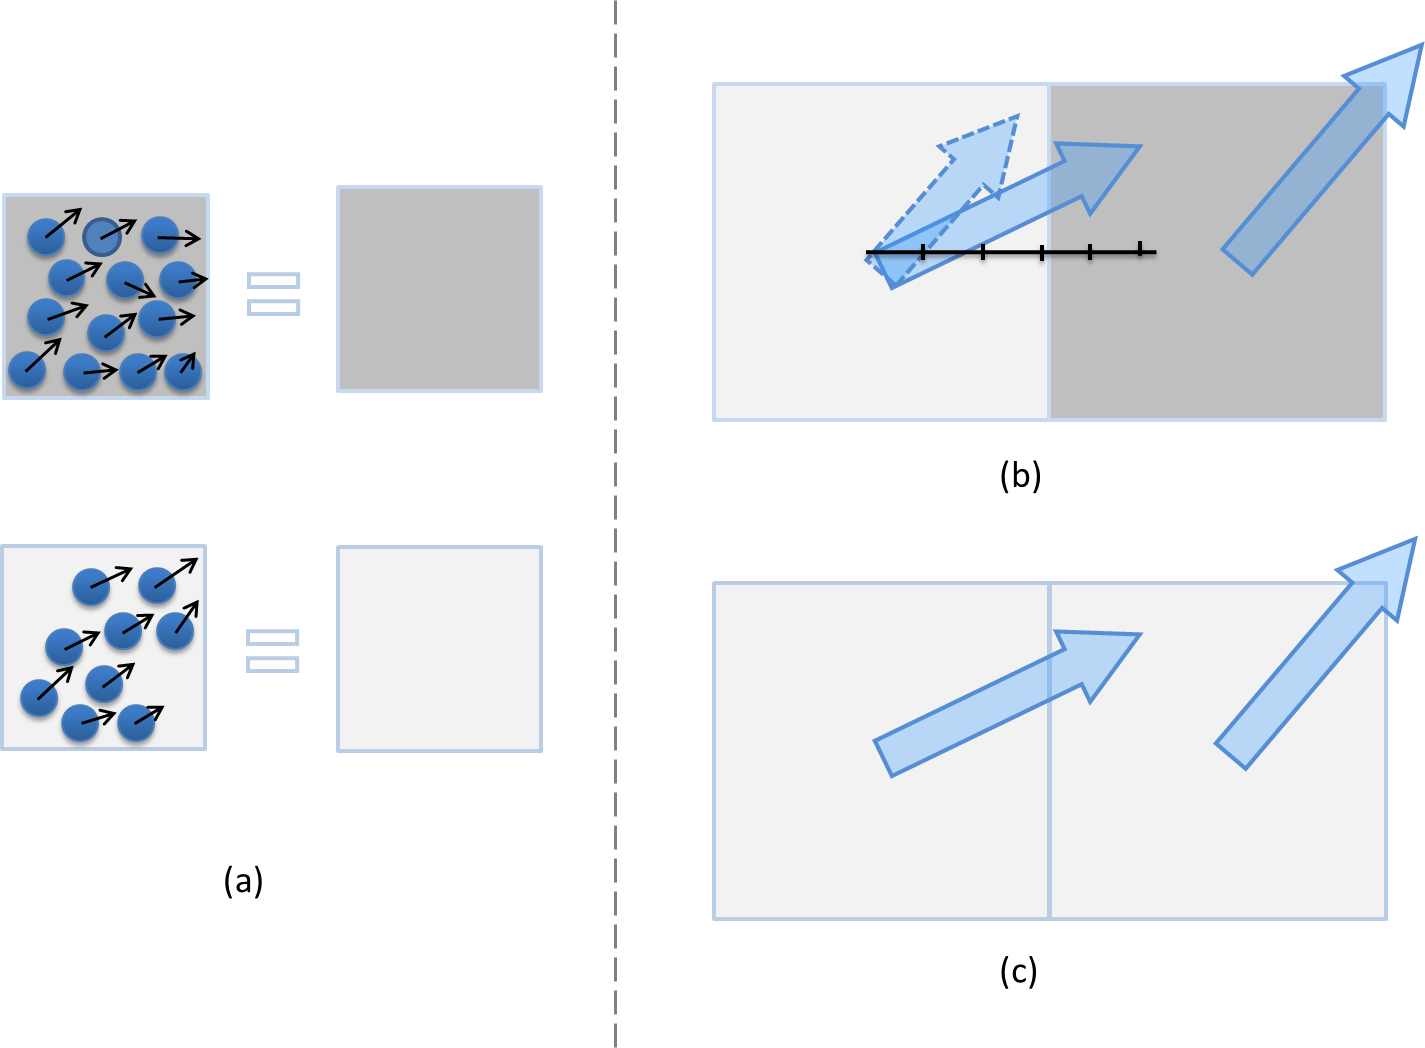
\includegraphics[width=3in]{images/fig_inter_grid_constraints}
  \caption{Sample illustration.}
\end{figure}

\section{Hybrid Crowd Simulation}
Continuous crowd methods and agent-based methods are both based on assumptions of agent number and crowd density(see \ref{Golas:2013}).
\begin{figure*}
  \centering
  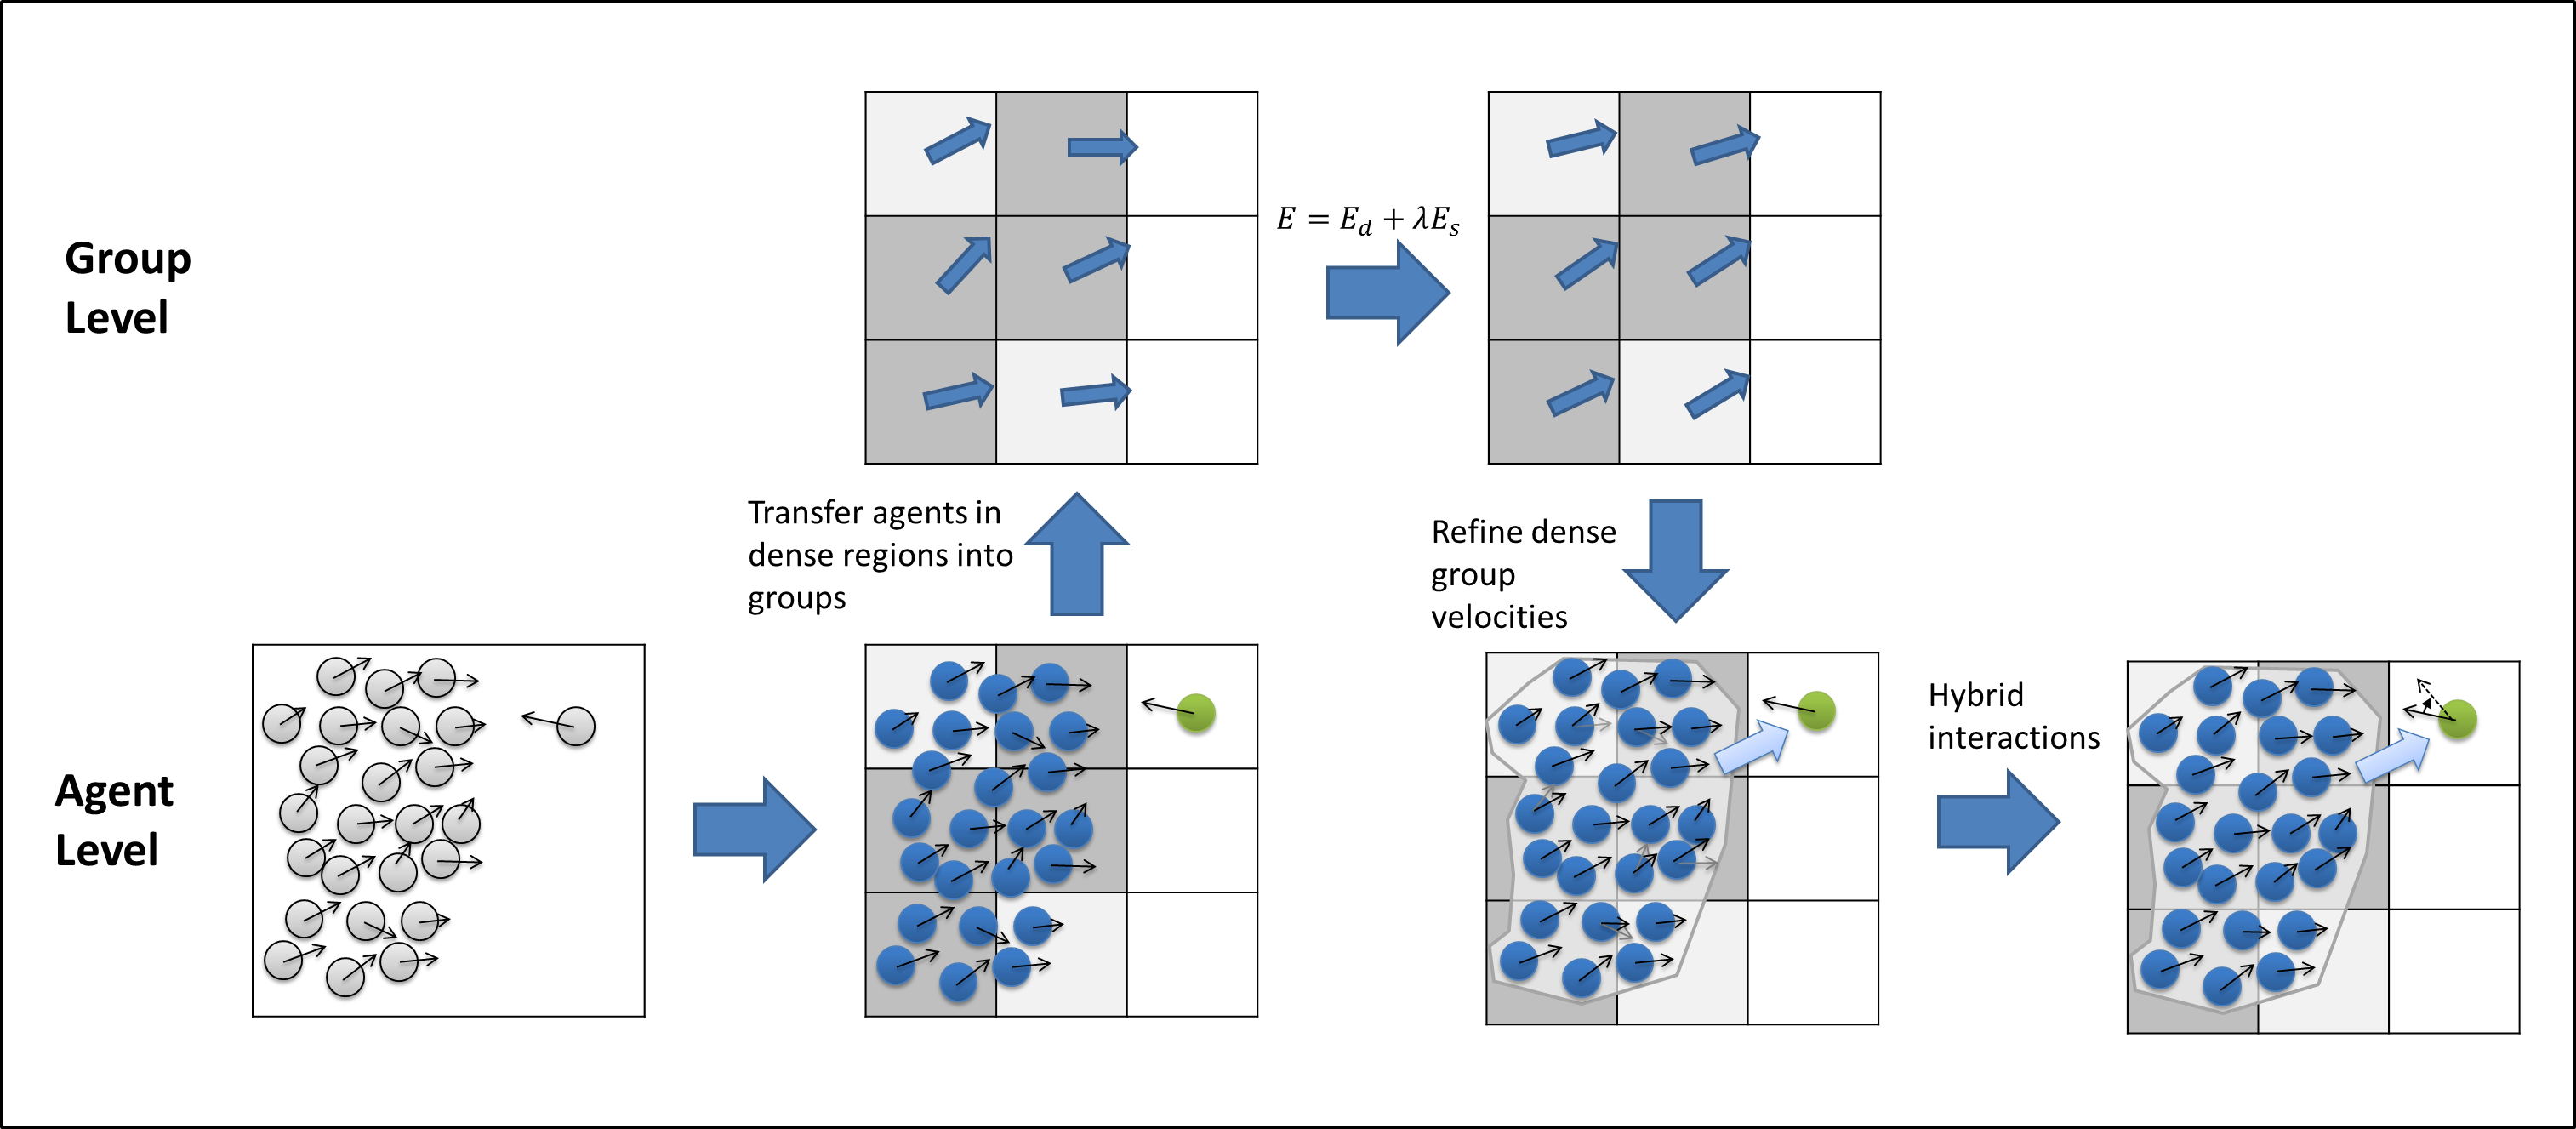
\includegraphics[width=6.4in]{images/pipeline}
  \caption{Sample illustration.}
\end{figure*}

\subsection{Dense Crowd Silhouette}

\subsection{Agent-based}
\begin{figure}
\centering
  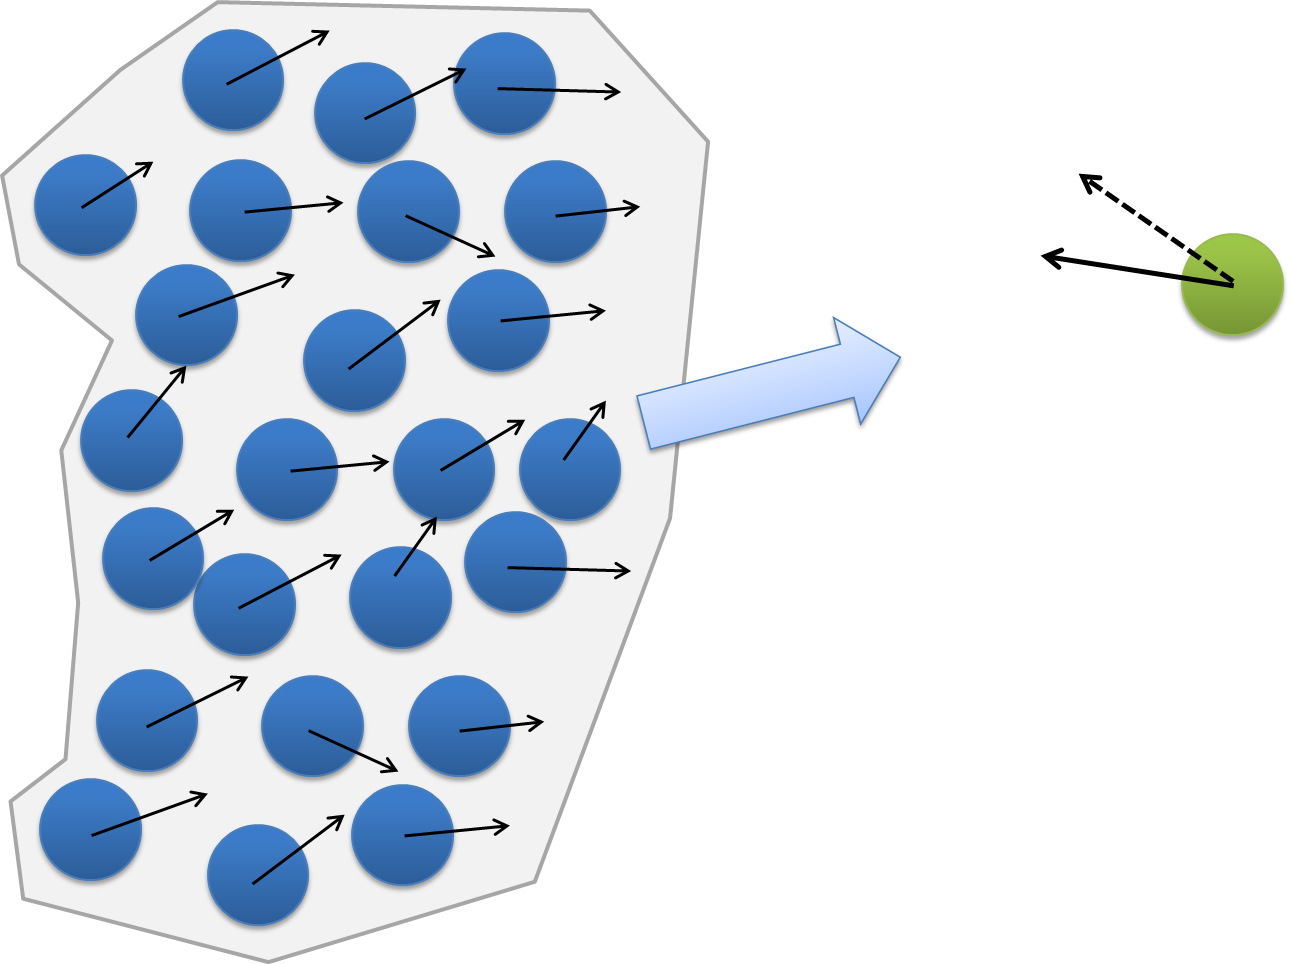
\includegraphics[width=1.6in]{images/agent_group_collision}
  \caption{Sample illustration.}
\end{figure}

%\bibliographystyle{eg-alpha}
\bibliographystyle{eg-alpha-doi}

\bibliography{reference}
\end{document}
